
%---------------------- % % % Personnalisation des couleurs % % % ----------- BLEU --------
\definecolor{couleurFonce}{RGB}{0,92,133} % Couleur du Code APOGEE
\definecolor{couleurClaire}{RGB}{100,151,186} % Couleur du fond de la bande
\definecolor{couleurTexte}{RGB}{255,255,255} % Couleur du texte de la bande
%------------------------------------------------------------------------------------------



%==========================================================================================
% Semestre 1
%==========================================================================================
\module[codeApogee={UE 11}, 
titre={Algorithmique et programmation 1}, 
CODEUE={2}, 
COURS={}, 
TD={}, 
TP={15}, 
CTD={45}, 
TOTAL={60}, 
SEMESTRE={Semestre 1}, 
COEFF={6}, 
ECTS={6}, 
MethodeEval={Contrôle continue et terminal}, 
ModalitesCCSemestreUn={CC et CT}, 
ModalitesCCSemestreDeux={CT}, 
%CalculNFSessionUne={$\frac{(CC+2*CT)}{3}$}, 
%CalculNFSessionDeux={CT}, 
NoteEliminatoire={}, 
nomPremierResp={Alexandre TESSIER}, 
emailPremierResp={Alexandre.TESSIER@univ-orleans.fr}, 
nomSecondResp={}, 
emailSecondResp={}, 
langue={Français}, 
nbPrerequis={0}, 
descriptionCourte={true}, 
descriptionLongue={true}, 
objectifs={true}, 
ressources={true}, 
bibliographie={false}] 
{
Unité obligatoire. 
}
{
Algorithmique élémentaire\,: expressions, variables, instructions, séquences, conditionnelles, boucles, tableaux, preuves, invariants, traduction dans un langage de programmation orienté objets.
} 
{} 
{\begin{itemize} 
 \ObjItem Maîtriser les concepts élémentaires de l\'algorithmique et être capable de les traduire dans un langages de programmation orienté objets. 
\end{itemize} 
} 
{Ressources} 
{Biblio} 
 
\vfill

%==========================================================================================
\module[codeApogee={UE 12}, 
titre={Atelier de l\'informaticien 1}, 
CODEUE={3}, 
COURS={}, 
TD={}, 
TP={}, 
CTD={24}, 
TOTAL={24}, 
SEMESTRE={Semestre 1}, 
COEFF={3}, 
ECTS={3}, 
MethodeEval={Contrôle continue et terminal}, 
ModalitesCCSemestreUn={CC et CT}, 
ModalitesCCSemestreDeux={CT}, 
%CalculNFSessionUne={$\frac{(CC+2*CT)}{3}$}, 
%CalculNFSessionDeux={CT}, 
NoteEliminatoire={}, 
nomPremierResp={Pierre RETY}, 
emailPremierResp={Pierre.RETY@univ-orleans.fr}, 
nomSecondResp={}, 
emailSecondResp={}, 
langue={Français}, 
nbPrerequis={0}, 
descriptionCourte={true}, 
descriptionLongue={true}, 
objectifs={true}, 
ressources={true}, 
bibliographie={false}] 
{
Unité obligatoire. 
} 
{
Présenter le système sous l\'angle de l\'utilisateur. Configuration de l\'environnement de travail de l\'informaticien 
} 
{} 
{\begin{itemize} 
 \ObjItem Être autonome dans la manipulation du système. 
\end{itemize} 
} 
{Ressources} 
{Biblio} 
 
\vfill

%==========================================================================================
\module[codeApogee={UE 13}, 
titre={Introduction au raisonnement mathématiques}, 
CODEUE={4}, 
COURS={}, 
TD={}, 
TP={}, 
CTD={60}, 
TOTAL={60}, 
SEMESTRE={Semestre 1}, 
COEFF={6}, 
ECTS={6}, 
MethodeEval={Contrôle continue et terminal}, 
ModalitesCCSemestreUn={CC et CT}, 
ModalitesCCSemestreDeux={CT}, 
%CalculNFSessionUne={$\frac{(CC+2*CT)}{3}$}, 
%CalculNFSessionDeux={CT}, 
NoteEliminatoire={}, 
nomPremierResp={François JAMES}, 
emailPremierResp={Francois.JAMES@univ-orleans.fr}, 
nomSecondResp={}, 
emailSecondResp={}, 
langue={Français}, 
nbPrerequis={0}, 
descriptionCourte={true}, 
descriptionLongue={true}, 
objectifs={true}, 
ressources={true}, 
bibliographie={false}] 
{
Unité obligatoire. 
} 
{
Logique naïve et manipulations ensemblistes. Injections, surjections. Structure d\'ordre, cas des réels, majorant, minorant, notion de borne supérieure. Approximations des réels : Q et D. Suites monotones et suites adjacentes. Structure vectorielle de R2 et R3. Sous-espaces vectoriels. Applications linéaires et matrices. Systèmes linéaires. Produit scalaire, produit vectoriel, produit mixte. 
} 
{} 
{\begin{itemize}
 \ObjItem Savoir mettre en \oe uvre un raisonnement mathématique de base. 
\end{itemize} 
} 
{Ressources} 
{Biblio} 
 
\vfill

%==========================================================================================
\module[codeApogee={UE 14}, 
titre={Suites et fonctions réelles}, 
CODEUE={1}, 
COURS={}, 
TD={}, 
TP={}, 
CTD={60}, 
TOTAL={60}, 
SEMESTRE={Semestre 1}, 
COEFF={6}, 
ECTS={6}, 
MethodeEval={Contrôle continue et terminal}, 
ModalitesCCSemestreUn={CC et CT}, 
ModalitesCCSemestreDeux={CT}, 
%CalculNFSessionUne={$\frac{(CC+2*CT)}{3}$}, 
%CalculNFSessionDeux={CT}, 
NoteEliminatoire={}, 
nomPremierResp={Jean-Philippe ANKER}, 
emailPremierResp={Jean-Philippe.ANKER@univ-orleans.fr}, 
nomSecondResp={}, 
emailSecondResp={}, 
langue={Français}, 
nbPrerequis={0}, 
descriptionCourte={true}, 
descriptionLongue={true}, 
objectifs={true}, 
ressources={true}, 
bibliographie={false}] 
{
Unité obligatoire. 
} 
{
Nombres complexes. Suites et fonctions. Fonctions usuelles. Continuité. Dérivabilité. Convexité. Étude de fonctions. 
} 
{} 
{\begin{itemize}
 \ObjItem Savoir mettre en \oe uvre un raisonnement mathématique de base. 
\end{itemize} 
} 
{Ressources} 
{Biblio} 
 
\vfill

%==========================================================================================
\module[codeApogee={UE 15}, 
titre={Arithmétique}, 
CODEUE={1}, 
COURS={}, 
TD={}, 
TP={}, 
CTD={24}, 
TOTAL={24}, 
SEMESTRE={Semestre 1}, 
COEFF={3}, 
ECTS={3}, 
MethodeEval={Contrôle continue et terminal}, 
ModalitesCCSemestreUn={CC et CT}, 
ModalitesCCSemestreDeux={CT}, 
%CalculNFSessionUne={$\frac{(CC+2*CT)}{3}$}, 
%CalculNFSessionDeux={CT}, 
NoteEliminatoire={}, 
nomPremierResp={Patrick MAHEUX}, 
emailPremierResp={Patrick.MAHEUX@univ-orleans.fr}, 
nomSecondResp={}, 
emailSecondResp={}, 
langue={Français}, 
nbPrerequis={0}, 
descriptionCourte={true}, 
descriptionLongue={true}, 
objectifs={true}, 
ressources={true}, 
bibliographie={false}] 
{
Unité obligatoire. 
} 
{
Divisibilité, théorèmes de Bézout et Gauss, décomposition en facteurs premiers. Exemples de structures : anneaux, corps. Congruences, structure de Z/nZ. Aperçu de ces notions dans le cadre de l\'anneau des fonctions polynômes.
} 
{} 
{\begin{itemize}
 \ObjItem Grâce aux exemples d\'arithmétiques élémentaires, découvrir l\'importance de quelques structures algébriques. 
\end{itemize} 
} 
{Ressources} 
{Biblio} 
 
\vfill

%==========================================================================================
\module[codeApogee={UE 16}, 
titre={Anglais 1}, 
CODEUE={1}, 
COURS={}, 
TD={25}, 
TP={}, 
CTD={}, 
TOTAL={25}, 
SEMESTRE={Semestre 1}, 
COEFF={3}, 
ECTS={3}, 
MethodeEval={Contrôle continue et terminal}, 
ModalitesCCSemestreUn={Contrôle continu}, 
ModalitesCCSemestreDeux={Contrôle terminal}, 
%CalculNFSessionUne={$\frac{(CC+2*CT)}{3}$}, 
%CalculNFSessionDeux={CT}, 
NoteEliminatoire={}, 
nomPremierResp={Murielle PASQUET}, 
emailPremierResp={Murielle.PASQUET@univ-orleans.fr}, 
nomSecondResp={}, 
emailSecondResp={}, 
langue={Français}, 
nbPrerequis={1}, 
descriptionCourte={true}, 
descriptionLongue={true}, 
objectifs={true}, 
ressources={true}, 
bibliographie={false}] 
{
Unité obligatoire. 
} 
{
Travail de compréhension et d’expression orale et écrite à partir de documents authentiques simples et/ou courts centrés sur le monde
universitaire anglo-saxon.
} 
{Niveau anglais baccalauréat LV1 ou LV2 ou équivalent.} 
{\begin{itemize} 
 \ObjItem Etre à même de préparer un projet de séjour d’études universitaires en pays anglophone dans une langue écrite et orale simple et suffisamment claire. 
\end{itemize} 
} 
{Ressources} 
{Biblio} 
 
\vfill

%==========================================================================================
\module[codeApogee={UE 17}, 
titre={Préparation au C2I}, 
CODEUE={1}, 
COURS={}, 
TD={24}, 
TP={}, 
CTD={}, 
TOTAL={24}, 
SEMESTRE={Semestre 1}, 
COEFF={3}, 
ECTS={3}, 
MethodeEval={Contrôle continue et terminal}, 
ModalitesCCSemestreUn={CC et CT}, 
ModalitesCCSemestreDeux={CT}, 
%CalculNFSessionUne={$\frac{(CC+2*CT)}{3}$}, 
%CalculNFSessionDeux={CT}, 
NoteEliminatoire={}, 
nomPremierResp={Laure KAHLEM}, 
emailPremierResp={Laure.KAHLEM@univ-orleans.fr}, 
nomSecondResp={}, 
emailSecondResp={}, 
langue={Français}, 
nbPrerequis={0}, 
descriptionCourte={true}, 
descriptionLongue={true}, 
objectifs={true}, 
ressources={true}, 
bibliographie={false}] 
{
Unité obligatoire. 
} 
{
S\'approprier son environnement de travail. Sécuriser son espace de travail local et distant. Pérenniser ses données.
Intégrer les règlementations concernant l\'utilisation des ressources numériques et les règles de bon usage du numérique. Maîtriser son identité numérique.
Maîtriser les fonctionnalités nécessaires à l\'élaboration et la structuration de documents complexes. Traiter des données chiffrées à l\'aide d\'un tableur.
Organiser la recherche d\'informations numériques.
} 
{} 
{\begin{itemize}
 \ObjItem Développer les compétences de base nécessaires à l\'usage des Technologies de l\'Information et de la Communication. 
\end{itemize} 
} 
{Ressources} 
{Biblio} 
 
\vfill


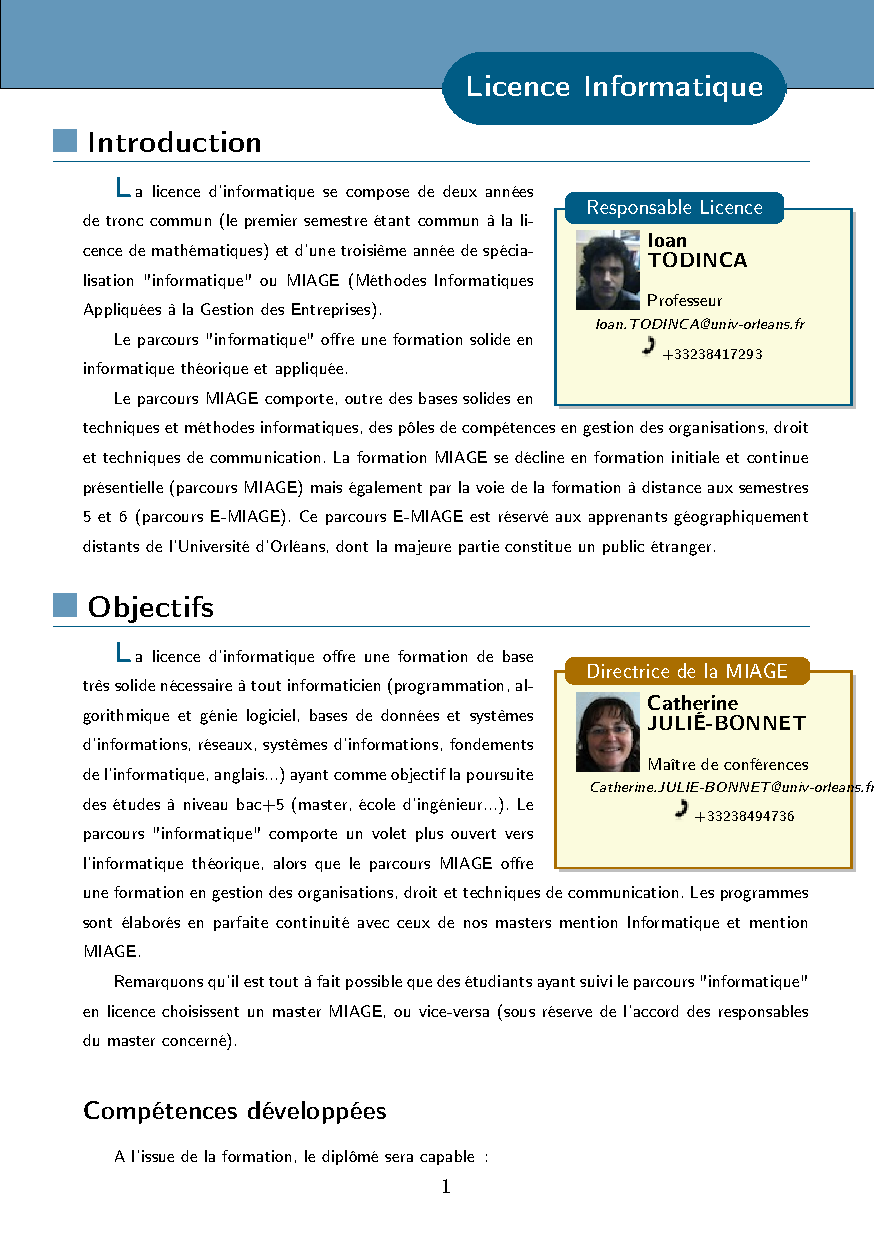
\includepdf[fitpaper,pages=-]{Preambule_Info_LicenceINFO_S2.pdf}

%==========================================================================================
% Semestre 2
%==========================================================================================
\module[codeApogee={UE 21}, 
titre={Algorithmique et programmation 2}, 
CODEUE={1}, 
COURS={}, 
TD={}, 
TP={}, 
CTD={60}, 
TOTAL={60}, 
SEMESTRE={Semestre 2}, 
COEFF={6}, 
ECTS={6}, 
MethodeEval={Contrôle continue et terminal}, 
ModalitesCCSemestreUn={CC et CT}, 
ModalitesCCSemestreDeux={CT}, 
%CalculNFSessionUne={$\frac{(CC+2*CT)}{3}$}, 
%CalculNFSessionDeux={CT}, 
NoteEliminatoire={}, 
nomPremierResp={Wadoud BOUSDIRA}, 
emailPremierResp={Wadoud.BOUSDIRA@univ-orleans.fr}, 
nomSecondResp={}, 
emailSecondResp={}, 
langue={Français}, 
nbPrerequis={1}, 
descriptionCourte={true}, 
descriptionLongue={true}, 
objectifs={true}, 
ressources={true}, 
bibliographie={false}] 
{
Unité obligatoire. 
} 
{
Algorithmique élémentaire\,: récursivité, objets, structures de données chaînées (listes, files, piles), notions élémentaires (allocation dynamique, chaînage des données), traduction dans un langage de programmation orienté objets.
} 
{UE Algorithmique et programmation 1} 
{\begin{itemize}
 \ObjItem Assimiler la programmation récursive d\'une part et d\'autre part, la définition et l\'utilisation de structures de données récursives. 
\end{itemize} 
} 
{Ressources} 
{Biblio} 
 
\vfill

%==========================================================================================
\module[codeApogee={UE 22}, 
titre={Outils mathématiques pour l\'informatique}, 
CODEUE={1}, 
COURS={}, 
TD={}, 
TP={}, 
CTD={50}, 
TOTAL={50}, 
SEMESTRE={Semestre 2}, 
COEFF={6}, 
ECTS={6}, 
MethodeEval={Contrôle continue et terminal}, 
ModalitesCCSemestreUn={CC et CT}, 
ModalitesCCSemestreDeux={CT}, 
%CalculNFSessionUne={$\frac{(CC+2*CT)}{3}$}, 
%CalculNFSessionDeux={CT}, 
NoteEliminatoire={}, 
nomPremierResp={Pierre RETY}, 
emailPremierResp={Pierre.RETY@univ-orleans.fr}, 
nomSecondResp={}, 
emailSecondResp={}, 
langue={Français}, 
nbPrerequis={1}, 
descriptionCourte={true}, 
descriptionLongue={true}, 
objectifs={true}, 
ressources={true}, 
bibliographie={false}] 
{
Unité obligatoire. 
} 
{
Logique des propositions et des prédicats. Étude des procédés de base des démonstrations mathématiques, sur des notions ensemblistes. Relations binaires, fermeture transitive, relations d\'équivalences, relations d\'ordre partiel. Récurrence forte sur la longueur des mots d\'un langage. Algèbre de Boole. Circuits. 
} 
{Les notions ensemblistes} 
{\begin{itemize}
 \ObjItem Comprendre et savoir écrire des démonstrations de mathématiques sur les ensembles et les relations binaires.
 \ObjItem Comprendre les relations d\'équivalences et les relations d\'ordre partiel.
 \ObjItem Être initié aux récurrences non-élémentaires, afin de pouvoir travailler sur l\'induction en 2ème année
 \ObjItem Être initié aux circuits booléens.
\end{itemize} 
} 
{Ressources} 
{Biblio} 
 
\vfill

%==========================================================================================
\module[codeApogee={UE 23}, 
titre={Modélisation}, 
CODEUE={1}, 
COURS={}, 
TD={}, 
TP={}, 
CTD={24}, 
TOTAL={24}, 
SEMESTRE={Semestre 2}, 
COEFF={3}, 
ECTS={3}, 
MethodeEval={Contrôle continue et terminal}, 
ModalitesCCSemestreUn={CC et CT}, 
ModalitesCCSemestreDeux={CT}, 
%CalculNFSessionUne={$\frac{(CC+2*CT)}{3}$}, 
%CalculNFSessionDeux={CT}, 
NoteEliminatoire={}, 
nomPremierResp={Frédéric LOULERGUE}, 
emailPremierResp={Frédéric.LOULERGUE@univ-orleans.fr}, 
nomSecondResp={}, 
emailSecondResp={}, 
langue={Français}, 
nbPrerequis={0}, 
descriptionCourte={true}, 
descriptionLongue={true}, 
objectifs={true}, 
ressources={true}, 
bibliographie={false}] 
{
Unité obligatoire. 
} 
{
Présentation simplifiée de techniques de modélisation et de leur mise en \oe uvre. 
} 
{} 
{\begin{itemize}
 \ObjItem Première approche des principes de modélisation des problèmes informatique. 
\end{itemize} 
} 
{Ressources} 
{Biblio} 
 
\vfill

%==========================================================================================
\module[codeApogee={UE 24}, 
titre={Projet informatique 1}, 
CODEUE={1}, 
COURS={}, 
TD={}, 
TP={24}, 
CTD={}, 
TOTAL={24}, 
SEMESTRE={Semestre 2}, 
COEFF={3}, 
ECTS={3}, 
MethodeEval={Contrôle continue et terminal}, 
ModalitesCCSemestreUn={Rapport et soutenance de projet}, 
ModalitesCCSemestreDeux={CT}, 
%CalculNFSessionUne={$\frac{(CC+2*CT)}{3}$}, 
%CalculNFSessionDeux={CT}, 
NoteEliminatoire={}, 
nomPremierResp={Wadoud BOUSDIRA}, 
emailPremierResp={Wadoud.BOUSDIRA@univ-orleans.fr}, 
nomSecondResp={}, 
emailSecondResp={}, 
langue={Français}, 
nbPrerequis={1}, 
descriptionCourte={true}, 
descriptionLongue={true}, 
objectifs={true}, 
ressources={true}, 
bibliographie={false}] 
{
Unité obligatoire. 
} 
{
Mise en \oe uvre des concepts vus dans les module d\'algorithmique 1 et 2. 
} 
{UE Algorithmique et programmation 1} 
{\begin{itemize} 
 \ObjItem Renforcer ses compétences et sa compréhension des principes d\'algorithmique et de programmation. 
\end{itemize} 
} 
{Ressources} 
{Biblio} 
 
\vfill

%==========================================================================================
\module[codeApogee={UE 25}, 
titre={Mathématiques}, 
CODEUE={1}, 
COURS={}, 
TD={}, 
TP={}, 
CTD={60}, 
TOTAL={60}, 
SEMESTRE={Semestre 2}, 
COEFF={6}, 
ECTS={6}, 
MethodeEval={Contrôle continue et terminal}, 
ModalitesCCSemestreUn={CC et CT}, 
ModalitesCCSemestreDeux={CT}, 
%CalculNFSessionUne={$\frac{(CC+2*CT)}{3}$}, 
%CalculNFSessionDeux={CT}, 
NoteEliminatoire={}, 
nomPremierResp={Prénom NOM}, 
emailPremierResp={Prenom.NOM@univ-orleans.fr}, 
nomSecondResp={}, 
emailSecondResp={}, 
langue={Français}, 
nbPrerequis={1}, 
descriptionCourte={true}, 
descriptionLongue={true}, 
objectifs={true}, 
ressources={true}, 
bibliographie={false}] 
{
Unité obligatoire. 
} 
{
Algèbre linéaire en dimension finie : Espaces et sous espaces vectoriels, bases, dimension, applications linéaires et matrices, théorème du rang. Systèmes linéaires. Diagonalisation. Fonctions réciproques et fonctions classiques. 
} 
{mathématiques de premier semestre ou équivalent} 
{\begin{itemize}
 \ObjItem Utiliser l\'algèbre linéaire générale, étude locale des fonctions 
\end{itemize} 
} 
{Ressources} 
{Biblio} 
 
\vfill

%==========================================================================================
\module[codeApogee={UE 26}, 
titre={Anglais 2}, 
CODEUE={1}, 
COURS={}, 
TD={25}, 
TP={}, 
CTD={}, 
TOTAL={25}, 
SEMESTRE={Semestre 2}, 
COEFF={3}, 
ECTS={3}, 
MethodeEval={Contrôle continue et terminal}, 
ModalitesCCSemestreUn={CC}, 
ModalitesCCSemestreDeux={CT}, 
%CalculNFSessionUne={$\frac{(CC+2*CT)}{3}$}, 
%CalculNFSessionDeux={CT}, 
NoteEliminatoire={}, 
nomPremierResp={Murielle PASQUET}, 
emailPremierResp={Murielle.PASQUET@univ-orleans.fr}, 
nomSecondResp={}, 
emailSecondResp={}, 
langue={Français}, 
nbPrerequis={1}, 
descriptionCourte={true}, 
descriptionLongue={true}, 
objectifs={true}, 
ressources={true}, 
bibliographie={false}] 
{
Unité obligatoire. 
} 
{
Travail de compréhension et d’expression orale et écrite à partir de documents authentiques simples et/ou courts centrés sur le monde universitaire anglo-saxon.
} 
{Avoir suivi l\'unité "Anglais 1" ou un volume d\'heures de formation équivalente.} 
{\begin{itemize} 
 \ObjItem Comprendre et s’exprimer de manière plus autonome dans des situations de séjour d’études universitaires en pays anglophone (niveau européen\,: B1).
\end{itemize} 
} 
{Ressources} 
{Biblio} 
 
\vfill

%==========================================================================================
\module[codeApogee={UE 27}, 
titre={Unité Libre}, 
CODEUE={1}, 
COURS={}, 
TD={22}, 
TP={}, 
CTD={}, 
TOTAL={22}, 
SEMESTRE={Semestre 2}, 
COEFF={3}, 
ECTS={3}, 
MethodeEval={Contrôle continue et terminal}, 
ModalitesCCSemestreUn={CC et CT}, 
ModalitesCCSemestreDeux={CT}, 
%CalculNFSessionUne={$\frac{(CC+2*CT)}{3}$}, 
%CalculNFSessionDeux={CT}, 
NoteEliminatoire={}, 
nomPremierResp={Scolarité des Sciences}, 
emailPremierResp={}, 
nomSecondResp={}, 
emailSecondResp={}, 
langue={Français}, 
nbPrerequis={0}, 
descriptionCourte={true}, 
descriptionLongue={true}, 
objectifs={true}, 
ressources={true}, 
bibliographie={false}] 
{
Unité obligatoire. 
} 
{
L\'unité Libre est à choisir, en début du semestre, parmi la centaine d\'enseignements dédiés à cet usage et offerts par toutes
les composantes de l\'université (Sciences, Droit-Economie-Gestion, Sport).\\
Voici quelques exemples d\'unités Libres\,:
\begin{itemize}
  \item Sport.
  \item Droit de l\'informatique.
  \item Problèmes économiques contemporains.
  \item Histoire du cinéma, histoire des arts.
  \item Enseigner : posture et identité professionnelles.
  \item Lecture critique du réchauffement climatique.
  \item Maîtriser son expression ; les enjeux de la communication orale : le corps, l\'espace, la voix.
\end{itemize} 
} 
{}
{\begin{itemize}
 \ObjItem Comprendre comment ce qu\'on apprend dans le cadre d\'un diplôme déjà très spécialisé s\'insère dans le large champ des connaissances
 et des savoirs auxquels on sera confronté dans son expérience professionnelle ou personnelle.
\end{itemize} 
} 
{La page du site de l\'université dédiée aux unités Libres: http://www.univ-orleans.fr/scolarite/inscriptions/?page=2} 
{Biblio} 
 
\vfill

%==========================================================================================
\module[codeApogee={UE 28}, 
titre={Projet personnel et professionnel}, 
CODEUE={1}, 
COURS={}, 
TD={}, 
TP={}, 
CTD={12}, 
TOTAL={12}, 
SEMESTRE={Semestre 3}, 
COEFF={3}, 
ECTS={3}, 
%MethodeEval={Contrôle continue et terminal}, 
ModalitesCCSemestreUn={Rapport et soutenance}, 
ModalitesCCSemestreDeux={Pas de 2nde session}, 
%CalculNFSessionUne={$\frac{(CC+2*CT)}{3}$}, 
%CalculNFSessionDeux={CT}, 
NoteEliminatoire={}, 
nomPremierResp={Wadoud BOUSDIRA}, 
emailPremierResp={Wadoud.BOUSDIRA@univ-orleans.fr}, 
nomSecondResp={}, 
emailSecondResp={}, 
langue={Français}, 
nbPrerequis={0}, 
descriptionCourte={true}, 
descriptionLongue={true}, 
objectifs={true}, 
ressources={true}, 
bibliographie={false}] 
{
Unité obligatoire.
} 
{
Explorer un métier, une fonction, un secteur d\'activité.
} 
{} 
{\begin{itemize}
 \ObjItem Choisir ses options en licence, envisager une poursuite d\'études en cours de licence et après la licence, et construire son projet professionnel. 
 \ObjItem Se confronter avec le milieu professionnel au travers d\'entretiens. 
\end{itemize} 
} 
{Ressources} 
{Biblio} 
 
\vfill

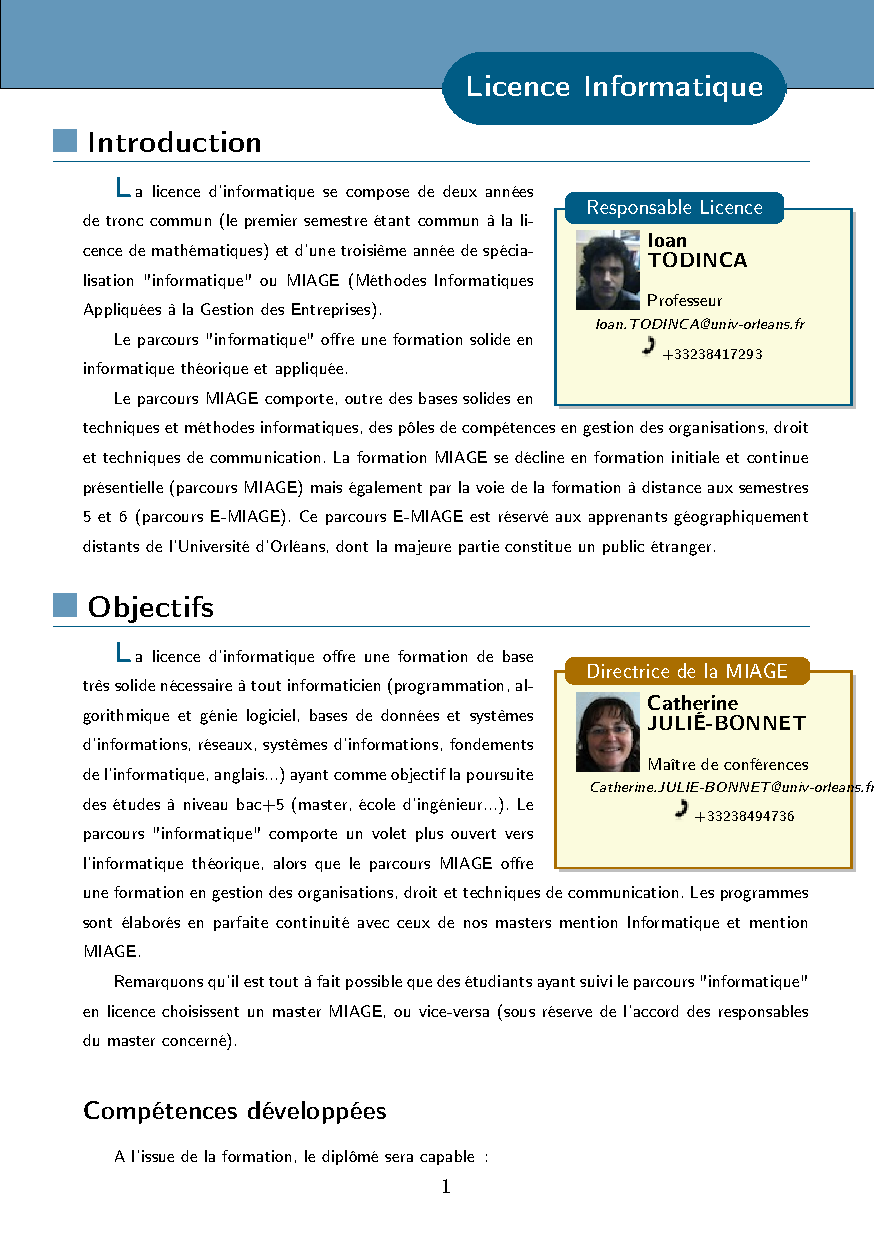
\includepdf[fitpaper,pages=-]{Preambule_Info_LicenceINFO_S3S4.pdf}

%==========================================================================================
% Semestre 3
%==========================================================================================
\module[codeApogee={UE 31}, 
titre={Algorithmique et programmation 3 (programmation orientée objet)}, 
CODEUE={1}, 
COURS={24}, 
TD={36}, 
TP={}, 
CTD={}, 
TOTAL={60}, 
SEMESTRE={Semestre 3}, 
COEFF={6}, 
ECTS={6}, 
MethodeEval={Contrôle continue et terminal}, 
ModalitesCCSemestreUn={CC et CT}, 
ModalitesCCSemestreDeux={CT}, 
%CalculNFSessionUne={$\frac{(CC+2*CT)}{3}$}, 
%CalculNFSessionDeux={CT}, 
NoteEliminatoire={}, 
nomPremierResp={Frédéric MOAL}, 
emailPremierResp={Frédéric.MOAL@univ-orleans.fr}, 
nomSecondResp={}, 
emailSecondResp={}, 
langue={Français}, 
nbPrerequis={1}, 
descriptionCourte={true}, 
descriptionLongue={true}, 
objectifs={true}, 
ressources={true}, 
bibliographie={false}] 
{
Unité obligatoire. 
} 
{
Présentation de l\'approche objet (valeurs + message), bases de conception/analyse objet. Notions de classes, méthodes, attributs, encapsulation, héritage (simple), interface, classe internes, exceptions... Mise en \oe uvre des interfaces graphiques et de la programmation événementielle.
} 
{Programmation impérative, algorithmes et structures de données (algorithmique et programmation 1 et 2).} 
{\begin{itemize}
 \ObjItem Maîtrise des bases de la conception et de la programmation objet. 
\end{itemize} 
} 
{Ressources} 
{Biblio} 
 
\vfill

%==========================================================================================
\module[codeApogee={UE 32}, 
titre={Bases de données et Internet}, 
CODEUE={1}, 
COURS={12}, 
TD={}, 
TP={24}, 
CTD={}, 
TOTAL={36}, 
SEMESTRE={Semestre 3}, 
COEFF={5}, 
ECTS={5}, 
MethodeEval={Contrôle continue et terminal}, 
ModalitesCCSemestreUn={CC et CT}, 
ModalitesCCSemestreDeux={CT}, 
%CalculNFSessionUne={$\frac{(CC+2*CT)}{3}$}, 
%CalculNFSessionDeux={CT}, 
NoteEliminatoire={}, 
nomPremierResp={Khalil DJELLOUL}, 
emailPremierResp={Khalil.DJELLOUL@univ-orleans.fr}, 
nomSecondResp={}, 
emailSecondResp={}, 
langue={Français}, 
nbPrerequis={1}, 
descriptionCourte={true}, 
descriptionLongue={true}, 
objectifs={true}, 
ressources={true}, 
bibliographie={false}] 
{
Unité obligatoire. 
} 
{
Architecture LAMP (Linux, Apache, MySQL, PHP). Modélisation d\'une base de donnée\,: modélisation conceptuelle (entité-association) \,; modélisation logique (relationnelle). Manipulation de données avec SQL. Structuration de pages web statiques et dynamiques. Réalisation d\'une application web dynamique (type PHP / MySQL). 
} 
{Maîtrise des bases de l\'algorithmique et de la programmation (pour la réalisation de 
l\'application web).} 
{\begin{itemize}
 \ObjItem Être à même de concevoir et réaliser une application web dynamique utilisant une base de données relationnelles. 
\end{itemize} 
} 
{Ressources} 
{Biblio} 
 
\vfill

%==========================================================================================
\module[codeApogee={UE 33}, 
titre={Atelier de l\'informaticien 2}, 
CODEUE={1}, 
COURS={12}, 
TD={}, 
TP={24}, 
CTD={}, 
TOTAL={36}, 
SEMESTRE={Semestre 3}, 
COEFF={4}, 
ECTS={4}, 
MethodeEval={Contrôle continue et terminal}, 
ModalitesCCSemestreUn={CC et CT}, 
ModalitesCCSemestreDeux={CT}, 
%CalculNFSessionUne={$\frac{(CC+2*CT)}{3}$}, 
%CalculNFSessionDeux={CT}, 
NoteEliminatoire={}, 
nomPremierResp={AbdelAli ED-DBALI}, 
emailPremierResp={AbdelAli.ED-DBALI@univ-orleans.fr}, 
nomSecondResp={}, 
emailSecondResp={}, 
langue={Français}, 
nbPrerequis={1}, 
descriptionCourte={true}, 
descriptionLongue={true}, 
objectifs={true}, 
ressources={true}, 
bibliographie={false}] 
{
Unité obligatoire.
} 
{
Présenter les outils nécessaires pour une utilisation approfondie du système dans le but d\'automatiser le processus de développement (shell, makefile, gestion de versions, etc).
} 
{Modules Algorithmique et programmation, Environnement Informatique.} 
{\begin{itemize}
 \ObjItem Automatiser la gestion du développement. 
\end{itemize} 
} 
{Ressources} 
{Biblio} 
 
\vfill

%==========================================================================================
\module[codeApogee={UE 34}, 
titre={Architecture des ordinateurs}, 
CODEUE={1}, 
COURS={12}, 
TD={12}, 
TP={6}, 
CTD={}, 
TOTAL={30}, 
SEMESTRE={Semestre 3}, 
COEFF={4}, 
ECTS={4}, 
MethodeEval={Contrôle continue et terminal}, 
ModalitesCCSemestreUn={CC et CT}, 
ModalitesCCSemestreDeux={CT}, 
%CalculNFSessionUne={$\frac{(CC+2*CT)}{3}$}, 
%CalculNFSessionDeux={CT}, 
NoteEliminatoire={}, 
nomPremierResp={Sophie ROBERT}, 
emailPremierResp={Sophie.ROBERT @univ-orleans.fr}, 
nomSecondResp={}, 
emailSecondResp={}, 
langue={Français}, 
nbPrerequis={1}, 
descriptionCourte={true}, 
descriptionLongue={true}, 
objectifs={true}, 
ressources={true}, 
bibliographie={false}] 
{
Unité obligatoire. 
} 
{
Étude du fonctionnement bas niveau d\'un ordinateur (couche matérielle). La représentation de l\'information (représentation binaire, standard IEEE 754). Les circuits séquentiels. La hiérarchie mémoire (mémoire RAM, adressage et réalisation à partir des bascules, cas particulier de la mémoire cache). L\'Unité centrale de traitement et son chemin de données. 
} 
{L\'algèbre de Boole et les circuits logiques.} 
{\begin{itemize}
 \ObjItem Compréhension des principes de base du fonctionnement d\'un ordinateur. 
\end{itemize} 
} 
{Ressources} 
{Biblio} 
 
\vfill

%==========================================================================================
\module[codeApogee={UE 35}, 
titre={Applications de l\'algèbre}, 
CODEUE={1}, 
COURS={}, 
TD={}, 
TP={}, 
CTD={48}, 
TOTAL={48}, 
SEMESTRE={Semestre 3}, 
COEFF={5}, 
ECTS={5}, 
MethodeEval={Contrôle continue et terminal}, 
ModalitesCCSemestreUn={CC et CT}, 
ModalitesCCSemestreDeux={CT}, 
%CalculNFSessionUne={$\frac{(CC+2*CT)}{3}$}, 
%CalculNFSessionDeux={CT}, 
NoteEliminatoire={}, 
nomPremierResp={Philippe GRILLOT}, 
emailPremierResp={Philippe.GRILLOT@univ-orleans.fr}, 
nomSecondResp={}, 
emailSecondResp={}, 
langue={Français}, 
nbPrerequis={1}, 
descriptionCourte={true}, 
descriptionLongue={true}, 
objectifs={true}, 
ressources={true}, 
bibliographie={false}] 
{
Unité obligatoire. 
} 
{
\begin{itemize}
\item Espaces vectoriels; bases; espaces supplémentaires; équations cartésiennes; applications linéaires; matrices d\'applications linéaires ( réelles et complexes); trace et déterminant d\'endomorphismes; calcul d\'inverses ( méthode du pivot de Gauss - méthode des cofacteurs); polynômes caractéristiques; valeurs propres ; vecteurs propres; diagonalisation; Théorème de Hamilton-Cayley; sous-espaces caractéristiques; lemme des noyaux.
\item Application : interpolation; résolution de systèmes linéaires, étude de suites récurrentes, résolution de systèmes différentiels, résolution d\'équations différentielles linéaires d\'ordre supérieur, exponentielle de matrices, trigonalisation. 
\end{itemize} 
} 
{niveau bac nécessaire, modules de première année souhaitables.} 
{\begin{itemize}
 \ObjItem Maîtrise des éléments d\'algèbre étudiés. 
\end{itemize} 
} 
{Ressources} 
{Biblio} 
 
\vfill

%==========================================================================================
\module[codeApogee={UE 36}, 
titre={Anglais 3}, 
CODEUE={1}, 
COURS={}, 
TD={25}, 
TP={}, 
CTD={}, 
TOTAL={25}, 
SEMESTRE={Semestre 3}, 
COEFF={3}, 
ECTS={3}, 
MethodeEval={Contrôle continue et terminal}, 
ModalitesCCSemestreUn={CC}, 
ModalitesCCSemestreDeux={CT}, 
%CalculNFSessionUne={$\frac{(CC+2*CT)}{3}$}, 
%CalculNFSessionDeux={CT}, 
NoteEliminatoire={}, 
nomPremierResp={Michèle CIMOLINO}, 
emailPremierResp={Michele.CIMOLINO@univ-orleans.fr}, 
nomSecondResp={}, 
emailSecondResp={}, 
langue={Français}, 
nbPrerequis={1}, 
descriptionCourte={true}, 
descriptionLongue={true}, 
objectifs={true}, 
ressources={true}, 
bibliographie={false}] 
{
Unité obligatoire. 
} 
{
Travail de compréhension et d’expression à partir de documents authentiques simples et/ou courts portant sur des innovations technologiques, des découvertes et avancées scientifiques.
} 
{Avoir suivi les unités Anglais 1 et 2 ou un volume d\'heures de formation équivalente} 
{\begin{itemize} 
 \ObjItem Découvrir les bases de l’anglais scientifique et les utiliser à l’écrit et à l’oral. 
\end{itemize} 
} 
{Ressources} 
{Biblio} 
 
\vfill

%==========================================================================================
\module[codeApogee={UE 37}, 
titre={Unité Libre}, 
CODEUE={1}, 
COURS={}, 
TD={24}, 
TP={}, 
CTD={}, 
TOTAL={24}, 
SEMESTRE={Semestre 3}, 
COEFF={3}, 
ECTS={3}, 
MethodeEval={Contrôle continue et terminal}, 
ModalitesCCSemestreUn={CC et CT}, 
ModalitesCCSemestreDeux={CT}, 
%CalculNFSessionUne={$\frac{(CC+2*CT)}{3}$}, 
%CalculNFSessionDeux={CT}, 
NoteEliminatoire={}, 
nomPremierResp={Scolarité des Sciences}, 
emailPremierResp={}, 
nomSecondResp={}, 
emailSecondResp={}, 
langue={Français}, 
nbPrerequis={0}, 
descriptionCourte={true}, 
descriptionLongue={true}, 
objectifs={true}, 
ressources={true}, 
bibliographie={false}] 
{
Unité obligatoire. 
} 
{
L\'unité Libre est à choisir, en début du semestre, parmi la centaine d\'enseignements dédiés à cet usage et offerts par toutes
les composantes de l\'université (Sciences, Droit-Economie-Gestion, Sport).\\
Voici quelques exemples d\'unités Libres\,:
\begin{itemize}
  \item Sport.
  \item Droit de l\'informatique.
  \item Problèmes économiques contemporains.
  \item Histoire du cinéma, histoire des arts.
  \item Enseigner : posture et identité professionnelles.
  \item Lecture critique du réchauffement climatique.
  \item Maîtriser son expression ; les enjeux de la communication orale : le corps, l\'espace, la voix.
\end{itemize} 
} 
{}
{\begin{itemize}
 \ObjItem Comprendre comment ce qu\'on apprend dans le cadre d\'un diplôme déjà très spécialisé s\'insère dans le large champ des connaissances
 et des savoirs auxquels on sera confronté dans son expérience professionnelle ou personnelle.
\end{itemize} 
} 
{La page du site de l\'université dédiée aux unités Libres: http://www.univ-orleans.fr/scolarite/inscriptions/?page=2} 
{Biblio} 
 
\vfill

%==========================================================================================
% Semestre 4
%==========================================================================================

\module[codeApogee={UE 41},
titre={Programmation fonctionnelle},
CODEUE={1},
COURS={24},
TD={36},
TP={},
CTD={},
TOTAL={60},
SEMESTRE={Semestre 4},
COEFF={6},
ECTS={6},
MethodeEval={Contrôle continue et terminal},
ModalitesCCSemestreUn={CC et CT},
ModalitesCCSemestreDeux={CT},
%CalculNFSessionUne={$\frac{(CC+2*CT)}{3}$},
%CalculNFSessionDeux={CT},
NoteEliminatoire={},
nomPremierResp={Frédéric DABROWSKI},
emailPremierResp={Frederic.DABROWSKI@univ-orleans.fr},
nomSecondResp={},
emailSecondResp={},
langue={Français},
nbPrerequis={1},
descriptionCourte={true},
descriptionLongue={true},
objectifs={true},
ressources={true},
bibliographie={false}]
{
Unité obligatoire.\\
Les langages de programmation fonctionnelle fortement typés conçus dans les années 80 sont utilisés dans
l\'enseignement depuis le milieu des années 90 et se diffusent de plus en plus dans l\'industrie.
Ils sont particulièrement appréciés par la productivité et la sûreté des programmes qu\'ils apportent. 
}
{
Présentation générale du langage fonctionnel utilisé. Expressions, valeurs et types de base Définitions locales, liaisons et environnements.
Expressions et valeurs fonctionnelles à une variable. Définitions globales, entrées-sorties, compilation en ligne de commande.
Fonctions d\'ordre supérieur. Filtrage, tuples. Polymorphisme et inférence de type. Fonctions récursives. Listes. Types composés\,:
type enregistrement, type somme (polymorphes & récursifs). Structures de données et algorithmes\,: tris, arbres binaires, arbres
binaires de recherche, arbres équilibrés.
}
{Mathématiques élémentaires dont preuve par récurrence. Utilisation élémentaire d\'un environnement Unix.}
{\begin{itemize}
 \ObjItem Prise en main d\'un des langages de programmation fonctionnelle et des notions de programmation associée.
 \ObjItem Développement d\'une application autonome complète.
\end{itemize}
}
{Ressources}
{Biblio}
 
\vfill

%==========================================================================================
\module[codeApogee={UE 42}, 
titre={Algorithmique et combinatoire des structures discrètes}, 
CODEUE={1}, 
COURS={24}, 
TD={36}, 
TP={}, 
CTD={}, 
TOTAL={50}, 
SEMESTRE={Semestre 4}, 
COEFF={6}, 
ECTS={6}, 
MethodeEval={Contrôle continue et terminal}, 
ModalitesCCSemestreUn={CC et CT}, 
ModalitesCCSemestreDeux={CT}, 
%CalculNFSessionUne={$\frac{(CC+2*CT)}{3}$}, 
%CalculNFSessionDeux={CT}, 
NoteEliminatoire={}, 
nomPremierResp={Mathieu LIEDLOFF}, 
emailPremierResp={Mathieu.LIEDLOFF@univ-orleans.fr}, 
nomSecondResp={}, 
emailSecondResp={}, 
langue={Français}, 
nbPrerequis={1}, 
descriptionCourte={true}, 
descriptionLongue={true}, 
objectifs={true}, 
ressources={true}, 
bibliographie={false}] 
{
Unité obligatoire.
} 
{
Dénombrement. Relation d\'ordre partiel : calcul de la fermeture transitive, tri topologique. Graphes : parcours, plus court chemin, arbres recouvrants de poids minimum, flot. 
} 
{algorithmique et programmation élémentaires} 
{\begin{itemize}
 \ObjItem Modélisation et résolution de problèmes à l\'aide de structures discrètes. 
\end{itemize} 
} 
{Ressources} 
{Biblio} 
 
\vfill

%==========================================================================================
\module[codeApogee={UE 43}, 
titre={Probabilités}, 
CODEUE={1}, 
COURS={}, 
TD={}, 
TP={}, 
CTD={48}, 
TOTAL={48}, 
SEMESTRE={Semestre 4}, 
COEFF={5}, 
ECTS={5}, 
MethodeEval={Contrôle continue et terminal}, 
ModalitesCCSemestreUn={CC et CT}, 
ModalitesCCSemestreDeux={CT}, 
%CalculNFSessionUne={$\frac{(CC+2*CT)}{3}$}, 
%CalculNFSessionDeux={CT}, 
NoteEliminatoire={}, 
nomPremierResp={Jean-Baptiste GOUÉRÉ}, 
emailPremierResp={Jean-Baptiste.GOUERE@univ-orleans.fr}, 
nomSecondResp={}, 
emailSecondResp={}, 
langue={Français}, 
nbPrerequis={1}, 
descriptionCourte={true}, 
descriptionLongue={true}, 
objectifs={true}, 
ressources={true}, 
bibliographie={false}] 
{
Unité obligatoire. 
} 
{
Espace de probabilités et modélisation de phénomènes aléatoires. Probabilités conditionnelles; indépendance; probabilités composées; formule de Bayes. Variables aléatoires discrètes et continues; fonction de répartition et loi de probabilité. Moment:espérance, variance, écart-type. Couple de variables aléatoires, loi jointe, lois marginales. Indépendance. Loi des grands nombres , théorème de la limite centrée, tables. 
} 
{mathématiques niveau bac} 
{\begin{itemize} 
 \ObjItem (savoirs et compétences acquis)\,: 
 \ObjItem maîtriser les bases du calcul des probabilités 
\end{itemize} 
} 
{Ressources} 
{Biblio} 
 
\vfill

%==========================================================================================
\module[codeApogee={UE 44}, 
titre={Projet informatique 2 (Conception et projet)}, 
CODEUE={1}, 
COURS={12}, 
TD={}, 
TP={24}, 
CTD={}, 
TOTAL={36}, 
SEMESTRE={Semestre 4}, 
COEFF={5}, 
ECTS={5}, 
MethodeEval={Réalisation d\'une application.}, 
ModalitesCCSemestreUn={Rapport et soutenance de projet}, 
ModalitesCCSemestreDeux={Pas de 2nde session}, 
%CalculNFSessionUne={$\frac{(CC+2*CT)}{3}$}, 
%CalculNFSessionDeux={CT}, 
NoteEliminatoire={}, 
nomPremierResp={Jean Michel COUVREUR}, 
emailPremierResp={Jean-Michel.COUVREUR@univ-orleans.fr}, 
nomSecondResp={}, 
emailSecondResp={}, 
langue={Français}, 
nbPrerequis={1}, 
descriptionCourte={true}, 
descriptionLongue={true}, 
objectifs={true}, 
ressources={true}, 
bibliographie={false}] 
{
Unité obligatoire. 
} 
{
Éléments de gestion de projet et de modélisation. Réalisation d\'un projet suivi par petits groupes. 
} 
{Cours d\'algorithmique et de programmation des semestres précédents.} 
{\begin{itemize}
 \ObjItem Avoir acquis une première expérience du travail de groupe et de l\'organisation d\'un projet. 
\end{itemize} 
} 
{Ressources} 
{Biblio} 
 
\vfill

%==========================================================================================
\module[codeApogee={UE 45}, 
titre={Anglais 4}, 
CODEUE={1}, 
COURS={}, 
TD={24}, 
TP={}, 
CTD={}, 
TOTAL={24}, 
SEMESTRE={Semestre 4}, 
COEFF={3}, 
ECTS={3}, 
MethodeEval={Contrôle continue et terminal}, 
ModalitesCCSemestreUn={CC}, 
ModalitesCCSemestreDeux={CT}, 
%CalculNFSessionUne={$\frac{(CC+2*CT)}{3}$}, 
%CalculNFSessionDeux={CT}, 
NoteEliminatoire={}, 
nomPremierResp={Michèle CIMOLINO}, 
emailPremierResp={Michele.CIMOLINO@univ-orleans.fr}, 
nomSecondResp={}, 
emailSecondResp={}, 
langue={Français}, 
nbPrerequis={1}, 
descriptionCourte={true}, 
descriptionLongue={true}, 
objectifs={true}, 
ressources={true}, 
bibliographie={false}] 
{
Unité obligatoire. 
} 
{
Travail de compréhension et d’expression à partir de documents authentiques simples et/ou courts portant sur des innovations technologiques, des découvertes et avancées scientifiques. 
} 
{Avoir suivi l\'unité "Anglais 3" ou un volume d\'heures de formation équivalente.} 
{\begin{itemize} 
 \ObjItem Analyser dans une langue simple et cohérente les rapports entre science et société à l’écrit et à l’oral (niveau européen\,: B1+).
\end{itemize} 
} 
{Ressources} 
{Biblio} 
 
\vfill

%==========================================================================================
\module[codeApogee={UE 46.A}, 
titre={Bases du système comptable}, 
CODEUE={1}, 
COURS={}, 
TD={}, 
TP={}, 
CTD={30}, 
TOTAL={30}, 
SEMESTRE={Semestre 4}, 
COEFF={5}, 
ECTS={5}, 
MethodeEval={Contrôle continue et terminal}, 
ModalitesCCSemestreUn={CC et CT}, 
ModalitesCCSemestreDeux={CT}, 
%CalculNFSessionUne={$\frac{(CC+2*CT)}{3}$}, 
%CalculNFSessionDeux={CT}, 
NoteEliminatoire={}, 
nomPremierResp={Gilles LE FLOHIC}, 
emailPremierResp={Gilles.LE-FLOHIC@univ-orleans.fr}, 
nomSecondResp={}, 
emailSecondResp={}, 
langue={Français}, 
nbPrerequis={0}, 
descriptionCourte={true}, 
descriptionLongue={true}, 
objectifs={true}, 
ressources={true}, 
bibliographie={false}] 
{
Choisir cette unité ou l\'unité UE 46.B (Programmation impérative).
} 
{
Le plan comptable général, La notion de flux : Le compte \,; Principe de la partie double. Les documents comptables \,:
Le journal \,; Le compte de résultat \,; Le bilan.
La facturation. Le règlement des créances et des dettes \,: Banque, caisse ou CCP \,; Les effets de commerce. 
} 
{} 
{\begin{itemize}
 \ObjItem Compréhension des bases du système comptable. 
\end{itemize} 
} 
{Ressources} 
{Biblio} 
 
\vfill

%==========================================================================================
\module[codeApogee={UE 46.B}, 
titre={Programmation impérative}, 
CODEUE={1}, 
COURS={12}, 
TD={20}, 
TP={}, 
CTD={}, 
TOTAL={32}, 
SEMESTRE={Semestre 4}, 
COEFF={5}, 
ECTS={5}, 
MethodeEval={Contrôle continue et terminal}, 
ModalitesCCSemestreUn={CC et CT}, 
ModalitesCCSemestreDeux={CT}, 
%CalculNFSessionUne={$\frac{(CC+2*CT)}{3}$}, 
%CalculNFSessionDeux={CT}, 
NoteEliminatoire={}, 
nomPremierResp={Matthieu EXBRAYAT}, 
emailPremierResp={Matthieu.EXBRAYAT@univ-orleans.fr}, 
nomSecondResp={}, 
emailSecondResp={}, 
langue={Français}, 
nbPrerequis={1}, 
descriptionCourte={true}, 
descriptionLongue={true}, 
objectifs={true}, 
ressources={true}, 
bibliographie={false}] 
{
Choisir cette unité ou l\'unité UE 46.A (Bases du système comptable).
} 
{
Apprentissage d\'un langage impératif avec gestion explicite de la mémoire. Gestion de la mémoire\,: allocation dynamique, pointeurs génériques et typage, données multidimentionnelles, gestion automatique. Modularisation des programmes\,: des principes de modularité à l\'objets génériques vers le polymorphisme. Mécanismes de contrôle avancés\,: sauts non locaux, exceptions, application à la gestion des erreurs d\'exécution. 
} 
{Initiation la programmation, programmation objets} 
{\begin{itemize}
 \ObjItem Connaître en profondeur un langage impératif. 
 \ObjItem Maîtriser les questions de gestion de mémoire.
 \ObjItem Programmer des concepts avancés de programmation à partir d\'un langage impératif. 
\end{itemize} 
} 
{Ressources} 
{Biblio} 
 
\vfill



